% NOTE -- ONLY EDIT THE .Rnw FILE!!!  The .tex file is
% likely to be overwritten.
%
% \VignetteIndexEntry{RankAggreg Overview}
% \VignetteDepends{clValid}
% \VignetteKeywords{rank aggregation, Cross-Entropy Monte Carlo algorithm, Genetic algorithm, meta analysis}
% \VignettePackage{RankAggreg}




\documentclass[11pt]{article}
%\documentclass[article, shortnames]{jss}

%\setlength{\oddsidemargin}{0.25truein}
%\setlength{\evensidemargin}{0.25truein}
%\setlength{\textwidth}{6.0truein} \setlength{\topmargin}{0.25truein}
%\setlength{\textheight}{8.5truein} \setlength{\headsep}{0.0truein}
%\setlength{\headheight}{0.0truein} \setlength{\topskip}{10.0pt}
%\pagestyle{empty} 
%\baselineskip=0.6cm

\usepackage{amsmath,amssymb,amsfonts} % Typical maths resource packages
\usepackage{graphics}                 % Packages to allow inclusion of graphics
\usepackage{color}                    % For creating coloured text and background
\usepackage{hyperref}                 % For creating hyperlinks in cross references
\usepackage{relsize}
\usepackage[mathcal]{euscript}
\usepackage[round]{natbib}
\usepackage{Sweave}

\begin{document}

\author{Vasyl
  Pihur, Somnath Datta, and Susmita Datta \\ \\
Department of Bioinformatics and Biostatistics, University of
Louisville \\
\url{http://louisville.edu/~v0pihu01/} }

\title{\emph{RankAggreg}, an R package for weighted rank 
aggregation}

\maketitle

\tableofcontents
\begin{abstract}
Rank aggregation plays an important role in our daily lives. Ordered lists are ubiquitous
and we, consciously or unconsciously, attempt to make sense of them. Unfortunately, for more
complex problems, where either the number of lists is large or the lists are long or both,
the aggregation becomes more than a simple brainteaser, often requiring advanced
computational techniques. The \emph{RankAggreg} package provides two methods for combining the 
ordered lists: the Cross-Entropy method and the Genetic Algorithm. Two examples of rank aggregation are given in 
the manuscript, one a moderately large problem in the context of clustering and the other relatively difficult one 
in the context of meta-analysis of microarray experiments.

\end{abstract}

%\Keywords{rank aggregation, Cross-Entropy Monte Carlo algorithm, Genetic algorithm, meta analysis}


%\Address{
%Vasyl Pihur\\
%Department of Bioinformatics and Biostatistics\\
%School of Public Health and Information Sciences\\
%University of Louisville\\
%555 S Floyd St.\\
%Louisville, KY, USA 40292\\
%E-mail: \email{v0pihu01@louisville.edu}\\
%URL: \url{http://louisville.edu/~v0pihu01/}
%}
\section{Introduction}
\label{sec:intro}

If you had to fill out at least one survey in your life, there is a 
good chance that you were asked to rank a collection of items in the 
order of preference from the most favorable to the least favorable. 
Certain voting schemes, particularly the ones used in the past, required 
voters to rank all candidates, making the final decision based on the 
obtained ordered lists. Many statistical and data mining procedures 
applied to large amounts of biological data usually produce a list, 
ordered according to some importance measure, of biologically 
meaningful entities such as, for example, a list of genes from a 
microarray experiment indicative of the cancer status. These are 
just a few examples that illustrate the abundance of ordered lists 
in all aspects of our lives, both scientific and mundane.

Franklin D. Roosevelt once said that "there are as many opinions as 
there are experts" and, thus, as many ordered lists on any given 
subject. Rank aggregation techniques are indispensable tools for 
combining individual ordered lists into a single "super"-list 
reflective of the overall preference or importance within the 
population. The idea is quite simple and, ideally, everyone's 
opinion should be accounted for. Different rank aggregation schemes, 
however, differ greatly in the underlying philosophy, as well as 
mathematical complexity.

Two radically different philosophies on rank aggregation exist. The 
first one is based on the majoritarian principles and attempts to accommodate the "majority" 
of individual preferences putting less or no weight on the relatively infrequent ones. The final 
aggregate ranking is usually based on the number of pairwise wins between 
items within individual lists. If item "A" is ranked higher than 
item "B" more often than not, then item "A" should also be ranked 
higher than item "B" in the overall list. The second philosophical 
approach to rank aggregation seeks the consensus among 
individual ordered lists and is usually based on some form of rank 
averaging. It is possible that the two approaches will produce 
different aggregated lists if applied to the same problem.

Conceptually, rank aggregation techniques range from quite simple 
(based on rank average or on a number of pairwise wins) to fairly 
complex and may employ advanced computational methodologies to find 
a solution. Simple solutions are not necessarily desirable as they 
usually rely on "ad hoc" principles and lack any formal 
justification. Mathematical rigor brings certain satisfaction and 
"security" at the expense of increased complexity and intensive 
computation.

In this paper, we present an R \emph{RankAggreg} package which provides 
two distinct algorithms for rank aggregation: the Cross-Entropy Monte Carlo algorithm (CE) 
\cite{Rub99, Deb05} and the Genetic algorithm (GA) \cite{Gol89}. 
Both methods are available through the main function \emph{RankAggreg}. In addition, 
a brute force algorithm is also provided through the \emph{BruteAggreg} function which simply tries all possible
solutions and selects the one which is optimal. What is meant by "optimal" and how to find the "optimal" solution will
be the discussion of the next sections.

\section{Rank aggregation as an optimization problem}
If we are to cast the rank aggregation in the framework of an optimization problem, we first would need to define our
objective function. In this context, we would like to find a "super"-list which would be as "close" as possible to all individual 
ordered lists simultaneously. This is a natural requirement and the objective function, at least in its most abstract form, is very simple and intuitive
\begin{eqnarray*}
\Phi(\delta) = \sum_{i=1}^m w_id(\delta, L_i),
\end{eqnarray*}
where $\delta$ is a proposed ordered list of length $k=|L_i|$, $w_i$ is the importance weight associated with list $L_i$, $d$ is a distance function which will be discussed in details
below, and $L_i$ is the $i^{th}$ ordered list \cite{Pih07}. 

The idea is to find $\delta^*$ which would minimize the total distance between $\delta^*$ and $L_i$'s
\begin{eqnarray*}
\delta^*=arg \hspace{.1cm} min \, \sum_{i=1}^m w_id(\delta, L_i).
\end{eqnarray*}

Selecting the appropriate distance function $d$ which would measure the "distance" between ordered lists is very important and two choices of a
distance function are available: Spearman footrule distance and Kendall's tau distance. The two distances usually produce slightly different aggregated
lists which is mainly due to the differences in the two philosophical paradigms discussed in the Introduction (\ref{sec:intro}). Now let us take a closer look at 
how "distances" between ordered lists are measured.

\subsection{Spearman footrule distance}
Before defining the two distance measures, let us introduce some necessary notation. Let $M_i(1), \ldots, M_i(k)$
    be the scores associated with the ordered list $L_i$, where $M_i(1)$ is the best (can be the largest or the smallest depending on the context)
    score, $M_i(2)$ is the second best, and so on. Let $r^{L_i}(A)$ be the rank of $A$ in the list $L_i$ (1 means "best") 
    if $A$ is within the top $k$, and be equal to $k+1$, otherwise; $r^\delta(A)$ is defined likewise.

    The Spearman's footrule distance between $L_i$ and any ordered list $\delta$ can be defined as
    $$
    S(\delta, L_i)=\sum_{t \in L_i \cup \delta} |r^\delta(t)-r^{L_i}(t)|.
    $$
    It is nothing more than the summation of the absolute differences between the ranks of all unique
    elements from both ordered lists combined. It is rather a very intuitive metric for comparing two ordered
    lists of arbitrary length. The smaller the value of the metric, the more similar the lists. For Spearman's
    footrule distance, the maximum value when comparing two top-$k$ lists is $k(k+1)$ which is attained when the two
    lists have no elements in common.
    
The appeal of the Spearman footrule distance comes from its simplicity and it is adequate in many situations when the only
information available about the individual lists is the rank order of their elements. In a case when additional information which was
used to rank the lists in the first place is available, it would be beneficial and prudent to incorporate this information into
our aggregation scheme \cite{Pih07}. Even though in soccer a win is a win, a win by 5 goals is more "convincing" than a marginal victory secured by a penalty kick on the last minute 
of the game. The \emph{qualitative} difference in terms of ranks has an objective \emph{quantitative} difference underlying it. This is probably true in most cases.

Thus, we define the Weighted Spearman's footrule distance between $L_i$ and any ordered list $\delta$ which makes use of the quantitative information 
available in many cases. It is given by this weighted sum representation
    \begin{eqnarray*}
    WS(\delta, L_i)&=& \sum_{t \in L_i \cup \delta}
    |M(r^\delta(t))-M(r^{L_i}(t))| \times |r^\delta(t)-r^{L_i}(t)|.
    \end{eqnarray*}
One can intuitively think of $WS(\delta, L_i)$ in terms of sum of penalties for moving an arbitrary element of the list $L_i$, $t$, from the
    position $r^\delta(t)$ to another position $r^{L_i}(t)$ within the list (second term of the products) adjusted by the
    difference in scores between the two positions (first term). 
    
\subsection{Kendall's tau distance}

    The Kendall's tau distance takes a different approach at measuring the distance between two ordered lists. 
    It utilizes pairs of elements from the union of two lists and is defined
    $$
    K(\delta, L_i)=\sum_{t,u \in L_i \cup \delta} K^p_{tu},
    $$
    where
    $$
    K^p_{tu} =
    \begin{cases}
    0 & \textnormal{if $r^\delta(t)<r^\delta(u),r^{L_i}(t)<r^{L_i}(u)$ or
    $r^\delta(t)>r^\delta(u),r^{L_i}(t)>r^{L_i}(u)$} \\
    1 & \textnormal{if $r^\delta(t)>r^\delta(u),r^{L_i}(t)<r^{L_i}(u)$ or
    $r^\delta(t)<r^\delta(u),r^{L_i}(t)>r^{L_i}(u)$} \\
    p & \textnormal{if $r^\delta(t)=r^\delta(u)=k+1$ or $r^{L_i}(t)=r^{L_i}(u)=k+1$}.
    \end{cases}
    $$
    Here, $p \in [0,1]$ is a parameter that needs to be specified for Kendall's tau. If $p$ is set to 0,
    the maximum value that the distance can achieve is $k^2$ and
    this happens when the intersection of the two lists compared is an empty set. Intuitively, Kendall's
    tau can be thought about in the following way. If the two elements $t$ and $u$ have the same ordering in
    both lists, then no penalty is incurred (a good scenario). If the element $t$ precedes $u$ in the first list
    and $u$ precedes $t$ in the second list, then a penalty of 1 is imposed (a bad scenario). A case when both
    $t$ and $u$ do not appear in either one of the lists (their ranks are $k+1$) can be handled by selecting $p$
    on a spectrum ranging from very liberal (0) to very conservative (1). That is, if we have no knowledge of the
    relative position of $t$ and $u$ in one of the lists, we have several choices in the matter. We can either
    impose no penalty (0), full penalty (1), or a partial penalty ($0 < p < 1$). The following three choices are
    common: 0, 1, and 0.5. It is a matter of a philosophical taste as to which option one chooses. We use $p=0$ in
    the internal Kendall function of the package.

    Somewhat analogously to the Weighted Spearman distance, the Weighted Kendall's tau is defined by
    $$
    WK(\delta, L_i)=\sum_{t,u \in L_i \cup \delta} |M(r^{L_i}(t))-M(r^{L_i}(u))|\times K^p_{tu},
    $$
    in which the penalty imposed is adjusted by the absolute difference in the scores for elements $t$ and $u$.
    Here, $K^p_{tu}$ is defined identically as above.
    
    Normalization of scores from each list $L_i$ before computing $WS$ and $WK$ is necessary. The weights must
    be comparable otherwise disproportionately large or small weights can benefit a particular list and pull the
    "optimal" list $\delta^*$ towards it. A number of normalization schemes that map the scores from the real line to 
    the interval $[0,1]$ were considered. Unfortunately, most of them resulted in transformed scores occupying a 
    very narrow portion of the interval. We settled for a simple normalization which spread the scores "evenly" between 0 and 1
    \begin{eqnarray*}
   M_i^* = \frac{M_i-\min(M_i)}{\max(M_i)-\min(M_i)}, \hspace{1cm} i=1,\ldots,n.
    \end{eqnarray*}  
    
We would like to make one last comment on the reasons behind introducing weighted distance measures here. Quite obviously they are 
 motivated by the desire for a more efficient use of the data, in this case, the numerical scores which underlie the rankings. But 
 that is not their sole purpose. When using the original Spearman and Kendall distances we noticed that in many situations no clear
 winner exists as two or more ordered lists have the same objective function score due to the discrete nature of the ranks.
 This brought computational instability into the 
 iterative aggregation process. The algorithm would never converge but would simply oscillate between the two "best" lists, understandably not knowing
 which one to pick. When continuous weights are used to adjust the discrete ranks, the possibility of such ties is almost eliminated and the
 algorithm is much more computationally stable. In addition, we obtain a clear winner in an objective way.  
    
\section{Cross-Entropy Monte Carlo algorithm}
        Due to practical considerations and computational convenience, we represent an ordered list as an        
        $(X)_{n\times k}$ random matrix
        whose entries are 0 or 1 with the constraints of its columns
        summing up to 1 and its row summing to at most 1. Here, $n$ is the total number of unique elements in
        all ordered lists to be combined and $k$ is usually the length of ordered lists (but can be smaller if necessary).
        Under this setup, each realization of $X$, $x$, uniquely determines
        an ordered list of size $k$ by the position of 1's in each
        column from left to right \cite{Lin06}. For example, if the full list was
        $(A, B, C)$, a $3\times 3$ matrix
        \begin{equation*}
        x=
        \begin{bmatrix}
        0 & 1 & 0\\
        0 & 0 & 1\\
        1 & 0 & 0
        \end{bmatrix}
        \end{equation*}
        would translate into a candidate list of $(C, A, B)$.

        Having defined $X$ as a matrix of size $n\times k$ with the
        two constraints regarding the sums of columns and rows, we
        thereby define the space of solutions, $\mathcal{X}$, to our minimization
        problem. It is of interest to find the minimum of the objective function $\Phi$
        over $\mathcal{X}$ and the corresponding $x$ at which that
        minimum is attained.

        Assume
        that $X$ comes from a pmf $P(x)$ that is indexed by the parameter
        matrix $(v)_{n\times k} = ((p_{jr}))$. More precisely, we assume that the joint distribution $P_v(X=x)$ satisfying the
        above two constraints is given by
        \begin{eqnarray*}
        P_v(x) &\propto & \prod_{j=1}^n
        \prod_{r=1}^k(p_{jr})^{x_{jr}} \\
                 &&\times I\left(\sum_{r=1}^k x_{jr} \le 1, 1 \le j \le n; \sum_{j=1}^n x_{jr} = 1, 1 \le r \le k\right)
        \end{eqnarray*}

        \noindent The CE algorithm proceeds in the following fashion:
        \begin{enumerate}
        \item{\textbf{Initialization}: Set $t=0$. Set the initial parameter matrix $v^0$ of the random
        distribution of $X$ to constant values; i.e., let each $p_{jr}^0=1/n$. Thus, at this
        stage, each of the $n$ unique elements has equal chances of being included in the overall lists of size
        $k$ for which the objective function $\Phi$ will be evaluated. This default behavior can
        be overridden by specifying the initial probability matrix $v1$ in the \emph{RankAggreg} function.}
		
        \item{\textbf{Sampling}: At each iteration $t$, draw a sample of size $N$ from $P_{v^t}(x)$. Find
        the corresponding top-$k$ lists $\delta_i$'s and the values of the objective
        function $\Phi(\delta_i)$. Sort the $\Phi(\delta_i)$'s in ascending
        order and find a $\rho$-quantile $y^t=\Phi_{([\rho N])}$, where $[a]$, for any
        real number $a$, is the integer part of $a$.}

        \item{\textbf{Updating}: Update the parameter vector as follows
        $$
        p_{jr}^{(t+1)}=(1-w)p_{jr}^t+w\frac{\sum^N_{i=1}I(\Phi(\delta_i) \le
        y^t)x_{ijr}}{\sum^N_{i=1}I(\Phi(\delta_i) \le y^t)},
        $$
        where $x_{ijr}$ is the value at the $jr^{th}$ position of the $i^{th}$ sample and
        $w$ is a weight parameter introduced to avoid convergence to a local
        maxima (specified by the \emph{weight} argument with the default value of .25).}
		
        \item{\textbf{Convergence}: The algorithm is stopped if the optimal list does not change in a 
        user-specified number of iterations. The default value is 7 for the CE algorithm 
        and it is specified by the \emph{convIn} argument.}
        \end{enumerate}

        The CE algorithm requires users to set a number of
        parameters. Convergence to a global optimal solution
        in many ways depends on the parameters chosen. It is recommended
        that the number of samples $N$ is to be set to at least
        $10k^2$ (in case, $n>>k$, $10kn$) and the rarity parameter $\rho$ is to be set to 0.01
        if $N$ is relatively large or 0.1 if $N$ is small (less
        than 100). 

\section{Genetic algorithm}
    Genetic algorithms are another set of tools suitable for solving
    complex combinatorial problems \cite{Gol89}. Their main advantage is their
    inherent simplicity in both conceptual understanding and software implementation.
    In our experience, the GA perform reasonably well for the aggregation problem but one 
    has to be careful with the selection of important parameters defining the rate at which
    the learning proceeds.
    
    As implemented in this package, the GA has the following steps:
 \begin{enumerate}
        \item{\textbf{Initialization:} Randomly select \emph{popSize} ordered lists of size $k$ which form the initial
        population of possible solutions to our optimization problem. The population size \emph{popSize} is important and, obviously,
        the larger the population size, the better chance of it containing, at some point, the optimal solution. It should ideally be
        a function of $k$ and the number of unique elements in the original ordered lists $L_i$, but computational feasibility has to be 
        considered here.}
        \item{\textbf{Selection:} Depending on which distance is used, compute the objective function for each member of the population.
        Then randomly select current members for the next generation using weighted
        random sampling where the weights are determined by the member's fitness (the objective function score).} 
        \item{\textbf{Cross-over:} The selected
        members are then crossed-over with the probability of \emph{CP} (the cross-over probability), i.e. two random ordered lists
        can swap their tails which start at a random position with the \emph{CP} probability. Only 1-point cross-overs are allowed.}       
        \item{\textbf{Mutation:} Crossing-over will allow only for the mixing of ordered lists but a rather
        drastic event is required to bring radically new solutions to the population pool. These are introduced by mutations which
        happen with the probability of MP (mutation probability). Thus, any list in the pool can randomly change one or
        more of its elements.}
        \item{\textbf{Convergence:} The algorithm is stopped if the "optimal" list remains optimal for \emph{convIn} consecutive
        generations (default is 30). To ensure that the algorithm stops running eventually, the maximum number of generations can
        be set in advance which will terminate the execution regardless of the first condition being true. If neither
        the maximum number of iterations has been reached nor the "optimal" list stayed untouched during the last
        \emph{convIn} generations, continue to step Selection.}
 \end{enumerate}
 
 As was mentioned previously, the choice of the parameters \emph{popSize}, \emph{CP}, and \emph{MP} is crucial for the success of the GA.
 If one is too conservative and selects small \emph{CP} and \emph{MP} probabilities, the GA will have a hard time exploring the 
 space of possible solutions in a reasonable time, particularly, when the space is extremely large. On the other hand,
 choosing large values for \emph{CP} and \emph{MP} will results in a "haste" decision, perhaps getting stuck in a local minimum
 without a chance to explore the whole search space. 
 

\section{Examples of rank aggregation}
    We present two rank different rank aggregation problems, one in the context of unsupervised learning where there
    is an intrinsic difficulty of choosing the best clustering algorithm for a particular problem, and the other one
    in the context of meta-analysis of different microarray cancer studies where the goal is to determine the combined
    set of genes indicative of cancer status. 
    
    To start using the \emph{RankAggreg} package, it must be loaded into R with the regular \emph{library()} function.
    Package documentation, examples, and additional information are available through \emph{help()} and \emph{vignette()} functions.
    
\begin{Schunk}
\begin{Sinput}
> library(RankAggreg)
\end{Sinput}
\end{Schunk}
\begin{Schunk}
\begin{Sinput}
> help(package = "RankAggreg")
> vignette("RankAggreg")
\end{Sinput}
\end{Schunk}

\subsection{Aggregation of clustering validation measures}
    Rank aggregation in the clustering context was introduced by \cite{Pih07}. Numerous clustering algorithms are available in R and other
    statistical and data mining software packages, each
    one having its relative strength and weaknesses in terms of how successfully they can handle certain types of data. Thus, it is often difficult to
    select the "best" algorithm for a particular clustering task. Validation (performance) measures come to rescue to some extent and offer an 
    objective way of ranking clustering algorithms according to their assessment of what a "good" clustering result is. 
    If $k$ clustering algorithms are validated with $m$ validation measures, $m$ ordered lists of size $k$ are produced as a result. Even though desirable,
    the order of clustering algorithms within each list is rarely the same.
    Rank aggregation is helpful in reconciling the ranks and producing the "super"-list which determines the overall winner and also ranks all
    clustering algorithms based on their performance as determined by all $m$ validation measures simultaneously.
    
    Clustering validation is implemented in the \emph{clValid} package \cite{Bro07}. After loading the package, we bring in a mouse microarray dataset
    available and select the first 100 genes from it.
    Assuming that those 100 genes form 5 natural clusters (this is a big assumption but it is not essential for the rank aggregation demonstration),
    we evaluate 10 clustering algorithms with 6 validation measures. Available clustering algorithms are: SOM (SM), SOTA (ST), FANNY (FN),
    K-Means(KM), PAM(PM), Hierarchical(HR), Agnes(AG), CLARA(CL), Diana(DI), and Model-based(MO). 
    Further details can be obtained from the clValid package documentation.
    
    
\begin{Schunk}
\begin{Sinput}
> library(clValid)
> data(mouse)
> express <- mouse[1:100, c("M1", "M2", "M3", 
+     "NC1", "NC2", "NC3")]
> rownames(express) <- mouse$ID[1:100]
> set.seed(100)
> result <- clValid(express, 5, clMethods = c("hierarchical", 
+     "fanny", "model", "kmeans", "sota", "pam", 
+     "clara", "agnes", "diana", "som"), validation = c("internal", 
+     "stability"))
\end{Sinput}
\end{Schunk}
    
    The \emph{result} object contains a $7\times10$ matrix of scores which measure the performance of the algorithms. 
    For each validation measure, 10 clustering algorithms can now be ranked based on these scores which 
    are sorted either in ascending or descending order depending on whether larger or smaller scores
    correspond to better performance under the measure. Here, the Dunn index and the Silhouette Width measure give higher scores 
    with better performance and for the other measures the smaller scores are desirable. 
    

    This is how the 7 ordered lists of 10 algorithms look like.
    
\begin{Schunk}
\begin{Soutput}
             1  2  3  4  5  6  7  8  9  10
APN          SM FN ST KM PM HR AG CL DI MO
AD           SM FN KM PM CL ST DI HR AG MO
ADM          FN SM ST KM CL PM DI HR AG MO
FOM          SM CL KM PM FN ST DI HR AG MO
Connectivity HR AG DI KM MO SM FN CL PM ST
Dunn         HR AG KM PM DI SM CL MO FN ST
Silhouette   HR AG KM SM CL PM ST DI FN MO
\end{Soutput}
\end{Schunk}
The underlying validation measures' scores are given below.
\begin{Schunk}
\begin{Soutput}
                  1      2      3      4      5      6
APN           0.106  0.122  0.148  0.152  0.170  0.171
AD            1.633  1.671  1.701  1.707  1.708  1.739
ADM           0.284  0.306  0.368  0.467  0.481  0.481
FOM           0.567  0.576  0.584  0.593  0.594  0.595
Connectivity 23.911 23.911 35.436 36.092 37.488 38.396
Dunn          0.171  0.171  0.119  0.112  0.111  0.110
Silhouette    0.389  0.389  0.379  0.360  0.354  0.346
                  7      8      9     10
APN           0.171  0.183  0.183  0.264
AD            1.834  1.852  1.852  2.496
ADM           0.574  0.628  0.628  0.847
FOM           0.605  0.676  0.676  0.800
Connectivity 38.821 39.582 39.840 49.934
Dunn          0.084  0.082  0.081  0.056
Silhouette    0.330  0.312  0.299  0.165
\end{Soutput}
\end{Schunk}

We can see that both SOM and Hierarchical clustering are performing quite well and each is ranked first by
three different validation measures. If we had to pick the overall winner, it would probably be SOM as it 
performs better overall. For this particular aggregation problem it is feasible to determine the best 
performer without resorting to advanced computational techniques, but it is rather difficult to obtain the overall 
ordered list in this case. Since the number of possible solutions is not that large in this case 
$(k!=10! = 3,628,800)$, it is feasible to use the brute force approach to find the optimal solution.
This can be done using the \emph{BruteAggreg} function provided in the package. Please note 
that even for this relatively small problem it takes hours to perform the necessary computations. The approach
is limited to toy examples only and should not be attempted if $k$ is larger than 10.



\begin{Schunk}
\begin{Sinput}
> BruteAggreg(res$ranks, 10, res$weights, "Spearman")
\end{Sinput}
\end{Schunk}
The best overall list as determine by trying all possible solutions with the weighted Spearman footrule distance is 
SM HR KM FN AG PM CL DI ST MO with the minimum objective function score of
5.552256. As expected, SOM and Hierarchical clustering are the top two performers, followed by the K-Means algorithm. 
We will now see if the CE algorithm can quickly discover the solution without resorting to an exhaustive search.


\begin{Schunk}
\begin{Sinput}
> (CEWS <- RankAggreg(res$ranks, 10, res$weights, 
+     seed = 123))
\end{Sinput}
\end{Schunk}

\begin{Schunk}
\begin{Soutput}
The optimal list is: 
        SM HR KM FN AG PM CL DI ST MO

  Algorithm:   CE
  Distance:    Spearman
  Score:       5.552256 
\end{Soutput}
\end{Schunk}
We get exactly the same solution in only 13 iterations and in about 40 seconds by examining mere 13000 potential candidates.
We ran the CE algorithm 20 times using the default values with 20 different seeds. Only 1 out of 20 times it failed to discover the 
correct solution, switching K-Means and SOM algorithms. 

To get a visual representation of the results, a convenient \emph{plot} function is provided. It takes the 
object returned by the \emph{RankAggreg} function as its first argument and outputs three side-by-side plots with useful information
on the convergence properties and the final ranking.

\begin{figure}[hp]
\begin{center}
\begin{Schunk}
\begin{Sinput}
> plot(CEWS)
\end{Sinput}
\end{Schunk}
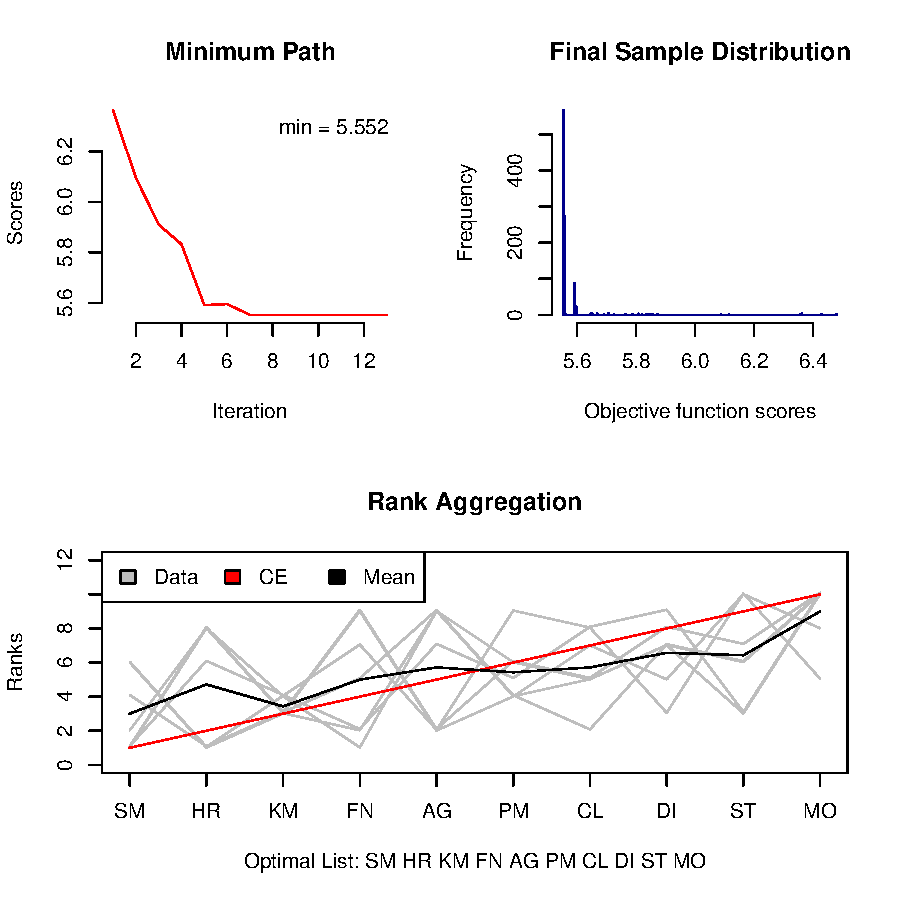
\includegraphics{RankAggreg-fig1}
\caption{Visual Representation of the aggregation results through the \emph{plot()} function. The first plot
in the top row shows the path of minimum values of the objective function over time. The global minimum is shown
in the top right corner. The histogram of the objective function scores at the last iteration is displayed in the
second plot. Looking at these two plots, one can get a general idea about the rate of convergence and the distribution
of candidate lists at the last iteration. The third plot at the bottom shows the individual lists and the obtained solution
along with optional average ranking.}
\end{center}
\end{figure}

Weighted Kendall's tau distance can also be used, though it is much more expensive to compute. If the \emph{verbose} argument
of the \emph{RankAggreg} function is set to TRUE (it is by default), R console window outputs information at each iteration
to keep the user updated. In addition, a plot similar to Figure 1 is shown and updated at each iteration to monitor convergence.

\begin{Schunk}
\begin{Sinput}
> (CEWK <- RankAggreg(res$ranks, 10, res$weights, 
+     "CE", "Kendall", seed = 123, verbose = FALSE))
\end{Sinput}
\end{Schunk}

\begin{Schunk}
\begin{Soutput}
The optimal list is: 
        KM SM PM FN HR AG CL DI ST MO

  Algorithm:   CE
  Distance:    Kendall
  Score:       1.241372 
\end{Soutput}
\end{Schunk}

Using the CE algorithm with the Kendall distance results in a different solution in which SOM is put in the second
position with K-Means occupying the first place. Maybe somewhat surprisingly, the Hierarchical clustering algorithm is ranked 
fifth despite the fact that it was ranked number 1 in 3 out of 7 lists. The rational explanation behind this decision is given by its
poor performance according to the other four measures which rank it towards the end.

The Genetic Algorithm can also be used with both the weighted Spearman and Kendall distances. Unfortunately, it seems to lack
the monotonicity property that the CE algorithm exhibits to some extent. This can be seen in the first plot of Figure 2.
Due to that fact, the convergence criteria needs to 
be stricter to avoid sporadic local solutions. The default value for the \emph{convIn} arguments for the GA is 30.

\begin{Schunk}
\begin{Sinput}
> (GAWS <- RankAggreg(res$ranks, 10, res$weights, 
+     "GA", "Spearman", seed = 123, verbose = FALSE))
\end{Sinput}
\end{Schunk}
\begin{Schunk}
\begin{Soutput}
The optimal list is: 
        SM HR KM FN AG PM CL DI ST MO

  Algorithm:   GA
  Distance:    Spearman
  Score:       5.552256 
\end{Soutput}
\end{Schunk}

\begin{Schunk}
\begin{Sinput}
> (GAWK <- RankAggreg(res$ranks, 10, res$weights, 
+     "GA", "Kendall", seed = 123, verbose = FALSE))
\end{Sinput}
\end{Schunk}
\begin{Schunk}
\begin{Soutput}
The optimal list is: 
        KM SM PM FN HR AG CL DI ST MO

  Algorithm:   GA
  Distance:    Kendall
  Score:       1.241372 
\end{Soutput}
\end{Schunk}

Both results agree with the ones obtained using the CE algorithm. 
Besides the jaggedness of the minimum path in the first plot, it is easy to notice that the GA 
algorithm takes significantly larger amount of cycles to converge. Even given that, the population distribution 
of the last generation is much more heterogeneous than that of the CE. 

\begin{figure}[hp]
\begin{center}
\begin{Schunk}
\begin{Sinput}
> plot(GAWS)
\end{Sinput}
\end{Schunk}
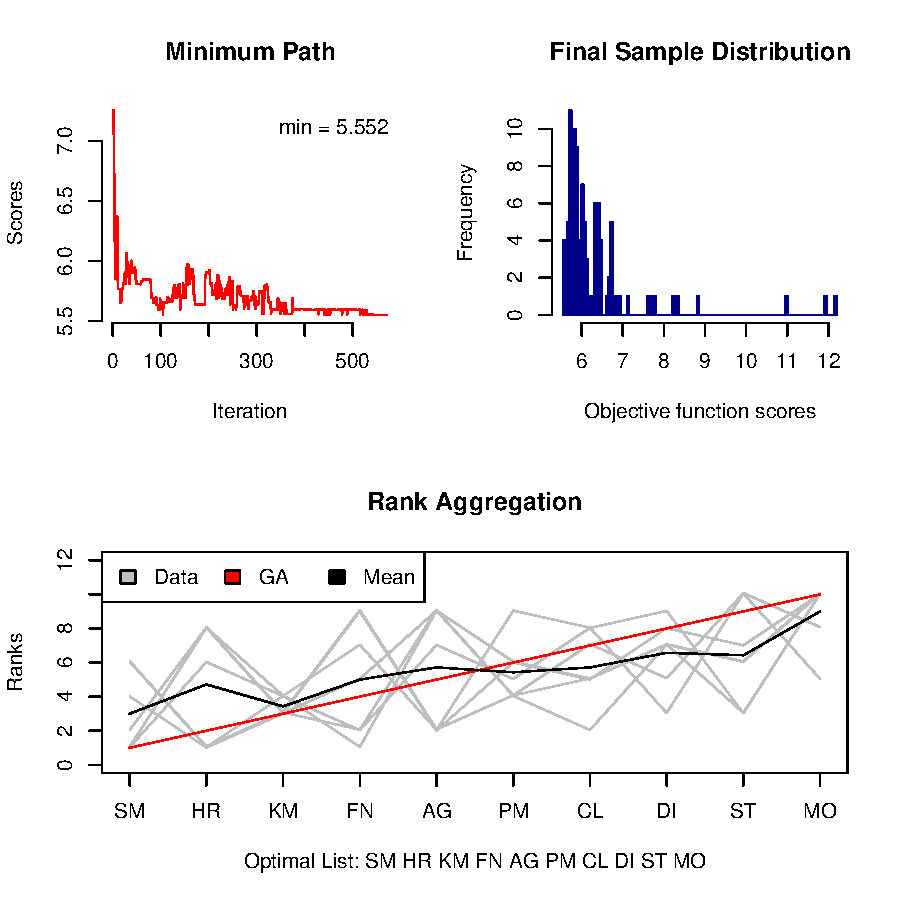
\includegraphics{RankAggreg-fig2}
\caption{Visual representation of rank aggregation using the GA algorithm with the Weighted Spearman distance.
}
\end{center}
\end{figure}

\subsection{Meta-analysis of microarray experiments}
Microarray cancer studies often attempt to identify genes related to a specific 
cancer. Their most common output is a list of genes ordered by corresponding
p-values. Different studies, even the ones analyzing the same cancer type (for
example, lung cancer), almost never produce identical gene lists. Meta-analysis
of multiple microarray studies is difficult, especially if different experimental
platforms have been used. Rank aggregation, however, avoids the issue of multiple
experimental conditions by dealing with the final product: the ordered list of genes.

Recently, we have carried out the meta-analysis of 20 microarray studies on
multiple cancers using the proposed rank aggregation algorithms \cite{Pih08}. 
Our goal was to identify genes which would be important in
development of multiple cancers. Further details on the rank aggregation details
can be found in the original article. 

Here, we present a smaller example described by \cite{Dec06} who used three different
Monte Carlo algorithms for rank aggregation of 5 prostate cancer microarray datasets.
Two experiments were conducted using the Affymetrix chip technology and the other three
studies used custom cDNA chips. Each individual study tried to identify genes which are
either up or down-regulated in prostate cancer patients, coming up with ordered lists of
upregualated genes shown in Table 1 (the lists appear in Table 4 in \cite{Dec06}).

\begin{Schunk}
\begin{Sinput}
> data(geneLists)
\end{Sinput}
\end{Schunk}

% latex table generated in R 2.6.2 by xtable 1.5-2 package
% Thu Feb 05 15:34:03 2009
\begin{table}[ht]
\begin{center}
\begin{tabular}{rlllll}
  \hline
 & Luo & Welsh & Dhana & True & Singh \\
  \hline
1 & HPN & HPN & OGT & AMACR & HPN \\
  2 & AMACR & AMACR & AMACR & HPN & SLC25A6 \\
  3 & CYP1B1 & 0ACT2 & FASN & NME2 & EEF2 \\
  4 & ATF5 & GDF15 & HPN & CBX3 & SAT \\
  5 & BRCA1 & FASN & UAP1 & GDF15 & NME2 \\
  6 & LGALS3 & ANK3 & GUCY1A3 & MTHFD2 & LDHA \\
  7 & MYC & KRT18 & 0ACT2 & MRPL3 & CANX \\
  8 & PCDHGC3 & UAP1 & SLC19A1 & SLC25A6 & NACA \\
  9 & WT1 & GRP58 & KRT18 & NME1 & FASN \\
  10 & TFF3 & PPIB & EEF2 & COX6C & SND1 \\
  11 & MARCKS & KRT7 & STRA13 & JTV1 & KRT18 \\
  12 & OS-9 & NME1 & ALCAM & CCNG2 & RPL15 \\
  13 & CCND2 & STRA13 & GDF15 & AP3S1 & TNFSF10 \\
  14 & NME1 & DAPK1 & NME1 & EEF2 & SERP1 \\
  15 & DYRK1A & TMEM4 & CALR & RAN & GRP58 \\
  16 & TRAP1 & CANX & SND1 & PRKACA & ALCAM \\
  17 & FM05 & TRA1 & STAT6 & RAD23B & GDF15 \\
  18 & ZHX2 & PRSS8 & TCEB3 & PSAP & TMEM4 \\
  19 & RPL36AL & ENTPD6 & EIF4A1 & CCT2 & CCT2 \\
  20 & ITPR3 & PPP1CA & LMAN1 & G3BP & SLC39A6 \\
  21 & GCSH & ACADSB & MAOA & EPRS & RPL5 \\
  22 & DDB2 & PTPLB & ATP6V0B & CKAP1 & RPS13 \\
  23 & TFCP2 & TMEM23 & PPIB & LIG3 & MTHFD2 \\
  24 & TRAM1 & MRPL3 & FM05 & SNX4 & G3BP2 \\
  25 & YTHDF3 & SLC19A1 & SLC7A5 & NSMAF & UAP1 \\
   \hline
\end{tabular}
\caption{Top-25 upregulated genes from 5 prostate microarray experiments.}
\end{center}
\end{table}
There are 89 unique genes in all 5 gene lists. The only gene that appears in all of them is HPN, while
genes AMACR, GDF15, and NME1 appear in 4 lists. 66 genes appear in just one list. The goal 
of rank aggregation is to combine these lists into the overall top-25 gene list which hopefully
would be more accurate than any individual list by itself. 

Since no p-values are reported, we will use the regular Spearman distance for both the CE and the GA algorithms.

\begin{Schunk}
\begin{Sinput}
> top25CE <- RankAggreg(geneLists, 25, seed = 100, 
+     rho = 0.01)
\end{Sinput}
\end{Schunk}

\begin{Schunk}
\begin{Soutput}
The optimal list is: 
        HPN AMACR GDF15 FASN NME2 UAP1 SLC25A6 0ACT2 KRT18 NME1
        EEF2 STRA13 GRP58 CANX SND1 ALCAM MRPL3 TMEM4 CCT2
        SLC19A1 PPIB FM05 ENTPD6 KRT7

  Algorithm:   CE
  Distance:    Spearman
  Score:       319.6 
\end{Soutput}
\end{Schunk}

The CE algorithm converges in 38 iterations with the minimum of 319.6. The overall list is perhaps not surprising, 
putting HPN in the first place, followed closely by the two other genes that appear in four lists. Using the GA
algorithm we get the similar results.

In case when there would be an indication that some microarray studies are more reliable than others, we could 
set the \emph{importance} parameter available in the \emph{RankAggreg} function to reflect these beliefs. By default,
it assigns equal weights to all ordered lists, but one, for example, could set importance=c(1,2,1,1,2) placing 
stronger emphasis on the Affymetrix arrays which are considered to have higher sensitivity rates.

\begin{Schunk}
\begin{Sinput}
> top25CEw <- RankAggreg(geneLists, 25, seed = 100, 
+     importance = c(1, 2, 1, 1, 2), rho = 0.01)
\end{Sinput}
\end{Schunk}

\begin{Schunk}
\begin{Soutput}
The optimal list is: 
        HPN AMACR 0ACT2 GDF15 FASN NME2 KRT18 SLC25A6 EEF2 UAP1
        CANX NME1 GRP58 SND1 STRA13 TMEM4 ALCAM PPIB NACA CCT2
        RPL5 SLC39A6 MTHFD2 MRPL3 SLC19A1

  Algorithm:   CE
  Distance:    Spearman
  Score:       295.4286 
\end{Soutput}
\end{Schunk}

This produces the combined list which is slightly
different from the one obtained treating all five studies equally.
The objective function score here is 295.43, being a little smaller
than 319.6. Clearly, OACT2 is ranked higher now (3rd) due to being
at the top (also 3rd) in the Welsh study which received more weight.
Similarly, the KRT18 gene moved up a couple spots due to being
present in both Welsh and Singh top lists which are both Affymetrix.

The GA algorithm can also be applied. We increase the maximum number
of iterations to allow for a longer evolution process. Increasing
the \emph{convIn} (converge in) argument to 50 will assure that we
do not stop the algorithm too soon.

\begin{Schunk}
\begin{Sinput}
> top25GA <- RankAggreg(geneLists, 25, seed = 100, 
+     method = "GA", maxIter = 3000, convIn = 50)
\end{Sinput}
\end{Schunk}

\begin{Schunk}
\begin{Soutput}
The optimal list is: 
        HPN AMACR SLC25A6 FASN NME2 GDF15 0ACT2 UAP1 KRT18 EEF2
        STRA13 NME1 MTHFD2 SND1 CANX GRP58 ALCAM TMEM4 PPIB CCT2
        SLC19A1 CBX3 SAT FM05 SNX4

  Algorithm:   GA
  Distance:    Spearman
  Score:       320.8 
\end{Soutput}
\end{Schunk}
The algorithm did not converge (due to setting a rather stringent
criteria) and was stopped after 3000 generations. The final list had
an objective function score of 320.8 which is slightly worse than
what we obtained using the CE algorithm. These lists are almost
identical in terms of which genes where included in the top 25 (22
genes are the same), but they are somewhat different in the actual
ordering. This should not come as a huge surprise, taking into consideration 
the enormous solution space. Both of the obtained lists are most likely very 
close to the true minimum solution.

\section{Discussion}
The \emph{RankAggreg} package provides an easy and convenient interface to handle complex
rank aggregation problems. It provides the user with two choices of methods for aggregation as
well as two different distance functions. The brute force approach is also available for
small-scale problems. A simple plot function helps to visualize the rank aggregation problem 
and the obtained solution. 

We would like to stress that using either the CE or the GA algorithms for large problems 
does not "guarantee" an optimal solution. Performance of both of these algorithms is quite 
sensitive to the tuning parameters, in particular the sample size \emph{N} for the CE algorithm and
the cross-over (CP) and mutation (MP) probabilities for the GA algorithm. The user is encouraged to run the
RankAggreg function several times. If different optimal lists are produced, increasing sample
size is probably necessary. Tuning additional parameters as discussed above may also
prevent local minima traps. That said, however, we are quite impressed by the ability of both
algorithms, the CE in particular, in discovering the optimal ordering of the elements in the
combined list.




{\small
  \bibliographystyle{abbrvnat}
  \bibliography{refs}
}

\end{document}

